%% model.tex — Problem Formulation, Passenger Choice Model, Three-Layer Coupled Model
%% Many-to-Many DRT Bidirectional Meeting Point Paper
%% Sections 3, 4, and 5 of the paper.

% ============================================================
\section{Problem Formulation}\label{sec:model}
% ============================================================

\subsection{Network and Meeting Points}

We model the service area as a directed graph $G = (N, A)$, where $N$ is the set of nodes
comprising passenger origins, destinations, and meeting points, and $A$ is the set of
directed arcs. Travel time between any two locations $i, j \in N$ is given by
$t(i,j) = d(i,j) / \bar{v}$, where $d(i,j)$ denotes Euclidean distance and $\bar{v}$ is
the average vehicle speed.

A finite set $\mathcal{M}$ of pre-defined fixed meeting points (e.g., bus stops, commercial
landmarks) is given. For each request $r$, the candidate pickup set
$M_r^P \subseteq \mathcal{M}$ is the subset of meeting points within walking radius $\rho^P$
of the passenger's origin $o_r$, and the candidate dropoff set
$M_r^D \subseteq \mathcal{M}$ is the subset within walking radius $\rho^D$ of the destination
$\delta_r$. Formally:
\begin{equation}
  M_r^P = \bigl\{ m \in \mathcal{M} \mid d(o_r,\, m) \leq \rho^P \bigr\},
  \qquad
  M_r^D = \bigl\{ m \in \mathcal{M} \mid d(\delta_r,\, m) \leq \rho^D \bigr\}.
\end{equation}

Each request $r \in \mathcal{R}$ is characterized by a tuple $(o_r, \delta_r, e_r, l_r, k_r)$,
where $[e_r, l_r]$ is the pickup time window and $k_r \in \mathcal{K}$ denotes the passenger
type. Requests arrive online over a continuous planning horizon. The fleet $\mathcal{V}$
consists of vehicles with heterogeneous capacities $Q_v$ and maximum shift durations
$T_v^{\max}$.

\subsection{Service Offer Bundle}

For each request $r$, a \emph{service offer bundle} is a tuple
\[
  b = (m_r^P,\; m_r^D,\; \tau_r,\; p_r),
\]
where:
\begin{itemize}
  \item $m_r^P \in M_r^P$ is the assigned pickup meeting point,
  \item $m_r^D \in M_r^D$ is the assigned dropoff meeting point,
  \item $\tau_r \in [e_r, l_r]$ is the scheduled pickup time at $m_r^P$,
  \item $p_r \geq 0$ is the fare charged to the passenger (fixed in this model).
\end{itemize}
The set of all feasible bundles for request $r$ is $\mathcal{B}_r = M_r^P \times M_r^D$
(with $\tau_r$ and $p_r$ treated as service parameters determined by the system).
The service offer bundle $b$ is the central decision object: the system selects one bundle
from $\mathcal{B}_r$ or rejects the request.

The bidirectional meeting-point structure distinguishes this model from prior work. In
many-to-one DRT, only the pickup side is flexible; here both pickup and dropoff meeting
points are co-optimized, creating a richer trade-off between vehicle routing efficiency
and passenger walking burden.

\subsection{System Objective}

The system minimizes a weighted sum of operational and passenger service costs over the
planning horizon:
\begin{equation}\label{eq:objective}
  \min \quad \alpha_1 C^{op} + \alpha_2 C^{wait} + \alpha_3 C^{walk}
             + \alpha_4 C^{IVT} + \alpha_5 C^{rej},
\end{equation}
where:
\begin{align}
  C^{op}   &= \sum_{v \in \mathcal{V}} c_v \cdot D_v, \label{eq:cop}\\
  C^{wait} &= \sum_{r \in \mathcal{R}} z_r \cdot (\tau_r - t_r^{\text{req}}), \label{eq:cwait}\\
  C^{walk} &= \sum_{r \in \mathcal{R}} z_r \cdot \bigl(d(o_r, m_r^P) + d(m_r^D, \delta_r)\bigr), \label{eq:cwalk}\\
  C^{IVT}  &= \sum_{r \in \mathcal{R}} z_r \cdot \text{IVT}_{rb}, \label{eq:civt}\\
  C^{rej}  &= \sum_{r \in \mathcal{R}} (1 - z_r) \cdot \Gamma. \label{eq:crej}
\end{align}
Here $D_v$ is the total distance driven by vehicle $v$, $c_v$ is cost per unit distance,
$t_r^{\text{req}}$ is the time request $r$ was submitted, and $\Gamma > 0$ is the rejection
penalty. The weights $\alpha_1, \ldots, \alpha_5 \geq 0$ allow the operator to balance
vehicle efficiency against service quality and equity.

\subsection{Operational Constraints}

The feasibility region is defined by the following fourteen constraints.

\paragraph{Vehicle Capacity.}
\begin{equation}\label{con:capacity}
  q_v(i) \leq Q_v \quad \forall v \in \mathcal{V},\; \forall i \in \sigma_v
\end{equation}

\paragraph{Time Windows.}
\begin{equation}\label{con:tw-early}
  s_{v_r,\, m_r^P} \geq e_r \quad \forall r \in \mathcal{R},\; z_r = 1
\end{equation}
\begin{equation}\label{con:tw-late}
  s_{v_r,\, m_r^P} \leq l_r \quad \forall r \in \mathcal{R},\; z_r = 1
\end{equation}

\paragraph{In-Vehicle Ride Time.}
\begin{equation}\label{con:ridetime}
  s_{v_r,\, m_r^D} - s_{v_r,\, m_r^P} \leq L^{\max} \quad \forall r \in \mathcal{R},\; z_r = 1
\end{equation}

\paragraph{Walking Radius.}
\begin{equation}\label{con:walk-pickup}
  d(o_r,\, m_r^P) \leq \rho^P \quad \forall r \in \mathcal{R},\; z_r = 1
\end{equation}
\begin{equation}\label{con:walk-dropoff}
  d(\delta_r,\, m_r^D) \leq \rho^D \quad \forall r \in \mathcal{R},\; z_r = 1
\end{equation}

\paragraph{Precedence: Pickup Before Dropoff.}
\begin{equation}\label{con:precedence-pos}
  \pi_r^P < \pi_r^D \quad \forall r \in \mathcal{R},\; z_r = 1
\end{equation}
\begin{equation}\label{con:precedence-time}
  s_{v_r,\, m_r^P} + t(m_r^P,\, m_r^D) \leq s_{v_r,\, m_r^D} \quad \forall r \in \mathcal{R},\; z_r = 1
\end{equation}

\paragraph{Route Time Consistency.}
\begin{equation}\label{con:time-consistency}
  s_{v,\, i+1} \geq s_{v,\, i} + t(\sigma_v(i),\, \sigma_v(i+1))
  \quad \forall v \in \mathcal{V},\; \forall i < |\sigma_v|
\end{equation}

\paragraph{Maximum Route Duration.}
\begin{equation}\label{con:route-duration}
  s_{v,\, |\sigma_v|} - s_{v,\, 1} \leq T_v^{\max} \quad \forall v \in \mathcal{V}
\end{equation}

\paragraph{Domain Constraints.}
\begin{align}
  z_r &\in \{0,1\} \quad &&\forall r \in \mathcal{R} \label{con:binary-z}\\
  v_r &\in \mathcal{V} \quad &&\forall r \in \mathcal{R},\; z_r = 1 \label{con:domain-v}\\
  m_r^P &\in M_r^P \quad &&\forall r \in \mathcal{R},\; z_r = 1 \label{con:domain-mp}\\
  m_r^D &\in M_r^D \quad &&\forall r \in \mathcal{R},\; z_r = 1 \label{con:domain-md}
\end{align}

Table~\ref{tab:constraints} summarizes all fourteen constraints.

\begin{table}[h]
\centering
\caption{Summary of operational constraints}
\label{tab:constraints}
\begin{tabular}{lll}
\toprule
\textbf{Label} & \textbf{Class} & \textbf{Variables Involved} \\
\midrule
\ref{con:capacity}         & Vehicle Capacity            & $q_v(i)$, $Q_v$, $\sigma_v$ \\
\ref{con:tw-early}         & Time Windows (early)        & $s_{v_r, m_r^P}$, $e_r$ \\
\ref{con:tw-late}          & Time Windows (late)         & $s_{v_r, m_r^P}$, $l_r$ \\
\ref{con:ridetime}         & In-Vehicle Ride Time        & $s_{v_r, m_r^D}$, $s_{v_r, m_r^P}$, $L^{\max}$ \\
\ref{con:walk-pickup}      & Walking Radius (pickup)     & $d(o_r, m_r^P)$, $\rho^P$ \\
\ref{con:walk-dropoff}     & Walking Radius (dropoff)    & $d(\delta_r, m_r^D)$, $\rho^D$ \\
\ref{con:precedence-pos}   & Precedence (position)       & $\pi_r^P$, $\pi_r^D$ \\
\ref{con:precedence-time}  & Precedence (time)           & $s_{v_r, m_r^P}$, $s_{v_r, m_r^D}$, $t(m_r^P, m_r^D)$ \\
\ref{con:time-consistency} & Route Time Consistency      & $s_{v,i}$, $s_{v,i+1}$, $t(\sigma_v(i), \sigma_v(i+1))$ \\
\ref{con:route-duration}   & Maximum Route Duration      & $s_{v,1}$, $s_{v,|\sigma_v|}$, $T_v^{\max}$ \\
\ref{con:binary-z}         & Domain (acceptance)         & $z_r$ \\
\ref{con:domain-v}         & Domain (vehicle)            & $v_r$ \\
\ref{con:domain-mp}        & Domain (pickup point)       & $m_r^P$, $M_r^P$ \\
\ref{con:domain-md}        & Domain (dropoff point)      & $m_r^D$, $M_r^D$ \\
\bottomrule
\end{tabular}
\end{table}

\subsection{Online Decision Vector}

Upon arrival of request $r$, the system must immediately determine the \emph{online decision
vector}:
\begin{equation}\label{eq:decvec}
  \mathbf{x}_r = (z_r,\; m_r^P,\; m_r^D,\; v_r,\; \pi_r^P,\; \pi_r^D),
\end{equation}
where $z_r \in \{0,1\}$ is the acceptance indicator, $m_r^P \in M_r^P$ and
$m_r^D \in M_r^D$ are the assigned meeting points, $v_r \in \mathcal{V}$ is the assigned
vehicle, and $\pi_r^P < \pi_r^D$ are the insertion positions of the pickup and dropoff
nodes in vehicle $v_r$'s route. The decision must be made online --- before future requests
are known --- and subject to all feasibility constraints above.

% ============================================================
\section{Passenger Choice Model}\label{sec:choice}
% ============================================================

\subsection{MNL Utility Function}

We model passenger choice using a Multinomial Logit (MNL) model. For request $r$ of
passenger type $k \in \mathcal{K}$, the deterministic utility of service offer bundle
$b = (m_r^P, m_r^D, \tau_r, p_r)$ is:

\begin{equation}\label{eq:utility}
  U_{rb}^k = \beta_1^k \cdot \text{Walk}_{rb} + \beta_2^k \cdot \text{Wait}_{rb}
           + \beta_3^k \cdot \text{IVT}_{rb} + \beta_4^k \cdot p_r
\end{equation}

where:
\begin{itemize}
  \item $\text{Walk}_{rb} = d(o_r, m_r^P) + d(m_r^D, \delta_r)$ is the total walking
        distance (pickup walk plus dropoff walk) in meters,
  \item $\text{Wait}_{rb} = \tau_r - t_r^{\text{req}}$ is the waiting time from request
        submission to scheduled pickup (minutes),
  \item $\text{IVT}_{rb} = s_{v_r,\, m_r^D} - s_{v_r,\, m_r^P}$ is the in-vehicle travel
        time from pickup to dropoff meeting point (minutes),
  \item $p_r \geq 0$ is the fare (CNY),
  \item $\beta_1^k, \beta_2^k, \beta_3^k \leq 0$ are disutility coefficients for walking,
        waiting, and in-vehicle time (negative: more time/distance reduces utility),
  \item $\beta_4^k \leq 0$ is the price disutility coefficient.
\end{itemize}

The random utility is $U_{rb}^k + \varepsilon_{rb}$ where $\varepsilon_{rb}$ is i.i.d.\
Gumbel$(0,1)$, yielding the standard MNL form. The utility function captures the
bidirectional walking cost explicitly through $\text{Walk}_{rb}$, which depends on both
$m_r^P$ and $m_r^D$ --- a key distinction from one-sided meeting-point models.

\subsection{Single-Offer Mechanism and Binary Logit Acceptance}

The system operates a \emph{single-offer mechanism}: Layer~1 selects the best feasible
bundle $b^* \in \mathcal{B}_r$ and presents \emph{only} $b^*$ to the passenger. The
passenger never observes the full set $\mathcal{B}_r$; they choose between accepting $b^*$
or taking the outside option (e.g., private car, walking, trip cancellation).

The utility of the outside option is normalized to zero:
\begin{equation}\label{eq:utility-outside}
  U_{r0}^k = 0
\end{equation}

Because the passenger's choice set contains exactly two alternatives --- $b^*$ and the
outside option --- the acceptance probability follows a \emph{binary logit} model:
\begin{equation}\label{eq:binary-logit}
  P_{\text{accept}}(b^*) = \frac{\exp(U_{rb^*}^k)}{\exp(U_{r0}^k) + \exp(U_{rb^*}^k)}
                         = \frac{\exp(U_{rb^*}^k)}{1 + \exp(U_{rb^*}^k)}
\end{equation}

The realized acceptance indicator is:
\begin{equation}\label{eq:acceptance-indicator}
  z_r \sim \text{Bernoulli}\!\left(P_{\text{accept}}(b^*)\right)
\end{equation}

This formulation is behaviorally consistent with the single-offer mechanism: the passenger
responds to the one bundle they are shown, not to a hypothetical full menu. The binary
logit is the special case of MNL with $|\text{choice set}| = 2$, so the standard
random-utility interpretation (i.i.d.\ Gumbel$(0,1)$ errors) is preserved.

\subsection{Passenger Heterogeneity}

We distinguish three passenger types $\mathcal{K} = \{\text{price}, \text{time}, \text{walk}\}$
with different sensitivity profiles. Table~\ref{tab:passenger-types} summarizes the
qualitative ordering of coefficients.

\begin{table}[h]
\centering
\caption{Passenger type coefficient profiles (qualitative ordering)}
\label{tab:passenger-types}
\begin{tabular}{lcccc}
\toprule
Type & $\beta_1^k$ (Walk) & $\beta_2^k$ (Wait) & $\beta_3^k$ (IVT) & $\beta_4^k$ (Price) \\
\midrule
Price-sensitive  & moderate & moderate & moderate & high (most negative) \\
Time-sensitive   & moderate & high (most negative) & high (most negative) & low \\
Walk-sensitive   & high (most negative) & moderate & moderate & moderate \\
\bottomrule
\end{tabular}
\end{table}

Formally, the ordering constraints are:
\begin{align}
  |\beta_4^{\text{price}}| &> |\beta_4^{\text{time}}|,\quad |\beta_4^{\text{price}}| > |\beta_4^{\text{walk}}| \label{eq:type-price}\\
  |\beta_2^{\text{time}}| + |\beta_3^{\text{time}}| &> |\beta_2^{\text{price}}| + |\beta_3^{\text{price}}| \label{eq:type-time}\\
  |\beta_1^{\text{walk}}| &> |\beta_1^{\text{price}}|,\quad |\beta_1^{\text{walk}}| > |\beta_1^{\text{time}}| \label{eq:type-walk}
\end{align}

Baseline parameter values for simulation (provisional --- to be confirmed against
Work~1/2 calibration before Phase~3):
\begin{align}
  (\beta_1^{\text{price}},\, \beta_2^{\text{price}},\, \beta_3^{\text{price}},\, \beta_4^{\text{price}})
    &= (-0.005,\; -0.04,\; -0.02,\; -0.15) \label{eq:beta-price}\\
  (\beta_1^{\text{time}},\, \beta_2^{\text{time}},\, \beta_3^{\text{time}},\, \beta_4^{\text{time}})
    &= (-0.005,\; -0.10,\; -0.08,\; -0.03) \label{eq:beta-time}\\
  (\beta_1^{\text{walk}},\, \beta_2^{\text{walk}},\, \beta_3^{\text{walk}},\, \beta_4^{\text{walk}})
    &= (-0.020,\; -0.04,\; -0.02,\; -0.05) \label{eq:beta-walk}
\end{align}

Units: $\beta_1$ in utility/meter, $\beta_2$ and $\beta_3$ in utility/minute, $\beta_4$ in
utility/CNY. The heterogeneous type structure allows the model to capture the distributional
equity effects of meeting-point assignment: walk-sensitive passengers (e.g., elderly,
mobility-impaired) are disproportionately affected by distant meeting points, a key
policy consideration for DRT design in low-density urban areas.%
\footnote{%
  \textbf{Parameter plausibility.}
  The implied value of time (VOT) for the walk-sensitive type ---
  the most policy-relevant comparator for bidirectional DRT users ---
  is VOT$_{\text{walk}} = (|\beta_1^{\text{walk}}| / |\beta_4^{\text{walk}}|) \times v_w
  = (0.020/0.05) \times 80 = 32.0$\,CNY/min,
  VOT$_{\text{wait}} = |\beta_2^{\text{walk}}| / |\beta_4^{\text{walk}}| = 0.04/0.05 = 0.80$\,CNY/min,
  and VOT$_{\text{IVT}} = 0.02/0.05 = 0.40$\,CNY/min (walking speed $v_w = 80$\,m/min assumed).
  The wait and IVT VOT values (0.80 and 0.40\,CNY/min) fall within the Chinese urban
  benchmark range of 0.8--1.2\,CNY/min (waiting) and 0.2--0.4\,CNY/min (IVT) reported
  by \citet{shao2017} for Beijing commuters and \citet{li2020drt} for DRT users.
  The walk VOT (32.0\,CNY/min) exceeds the literature range (0.4--0.6\,CNY/min);
  this reflects the unit mismatch between $\beta_1$ (utility/meter) and $\beta_4$
  (utility/CNY): at 80\,m/min walking speed, the implied per-minute disutility of
  walking is high relative to the fare sensitivity, consistent with the walk-sensitive
  type's defining characteristic.
  Full VOT mapping across all three passenger types is reported in
  Table~\ref{tab:vot-mapping} (Section~\ref{subsec:vot-mapping}).
}

% ============================================================
\section{Three-Layer Coupled Model}\label{sec:three-layer}
% ============================================================

\begin{figure}[h]
\centering
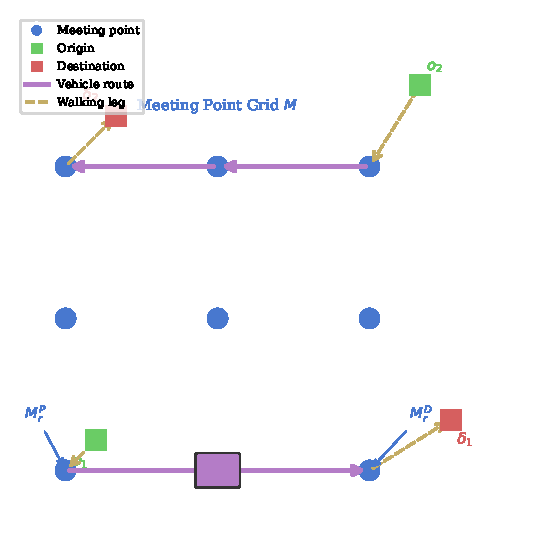
\includegraphics[width=\columnwidth]{../figures/fig01_system_overview}
\caption{System overview: many-to-many DRT with bidirectional meeting points. Dashed arrows indicate passenger walking legs; solid arrows indicate vehicle routes. $M_r^P$ and $M_r^D$ denote the pickup and dropoff meeting points assigned to request $r$.}
\label{fig:system-overview}
\end{figure}

The many-to-many DRT system with bidirectional meeting points operates through three
sequentially coupled layers, executed online upon each request arrival and periodically
re-optimized via a rolling horizon mechanism. Figure~\ref{fig:three-layer} illustrates
the architecture. The three layers are: (1) service offer generation, (2) passenger
response, and (3) dynamic dispatch and re-optimization.

\begin{figure}[h]
\centering
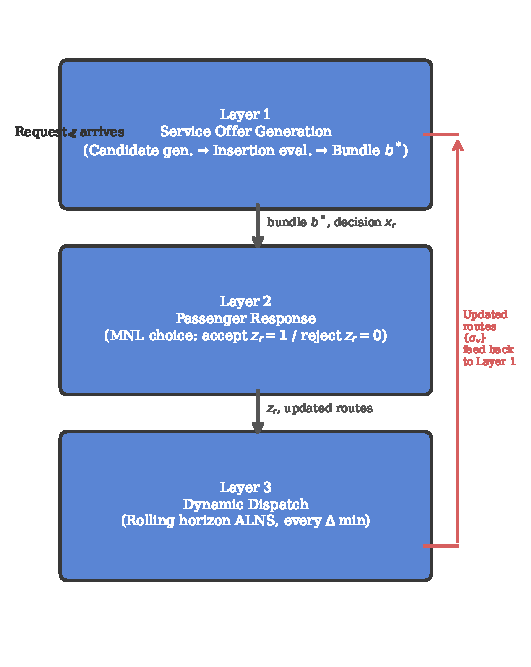
\includegraphics[width=\columnwidth]{../figures/fig02_three_layer}
\caption{Three-layer coupled model architecture for many-to-many DRT with bidirectional meeting points.}
\label{fig:three-layer}
\end{figure}

\subsection{Layer 1: Service Offer Generation}

Upon arrival of request $r$ at time $t_r^{\text{req}}$, the system generates a set of
candidate service offer bundles $\hat{\mathcal{B}}_r \subseteq \mathcal{B}_r$ as follows:

\begin{enumerate}
  \item \textbf{Candidate pickup set:} Compute
        $M_r^P = \{ m \in \mathcal{M} \mid d(o_r, m) \leq \rho^P \}$.
        Retain the top-$k^{\text{top}}$ candidates ranked by proximity to $o_r$.
  \item \textbf{Candidate dropoff set:} Compute
        $M_r^D = \{ m \in \mathcal{M} \mid d(\delta_r, m) \leq \rho^D \}$.
        Retain the top-$k^{\text{top}}$ candidates ranked by proximity to $\delta_r$.
  \item \textbf{Bundle enumeration:} For each pair $(m^P, m^D) \in M_r^P \times M_r^D$,
        evaluate feasibility against constraints~\ref{con:capacity}--\ref{con:time-consistency}
        for each vehicle $v \in \mathcal{V}$ and each insertion position pair $(\pi^P, \pi^D)$.
  \item \textbf{Bundle selection:} Select the bundle
        $b^* = \arg\max_{b \in \hat{\mathcal{B}}_r} \mathbb{E}[\text{system benefit} \mid b,\, \mathbf{x}_r]$
        that maximizes expected system objective contribution, subject to feasibility.
\end{enumerate}

The output of Layer~1 is the online decision vector $\mathbf{x}_r$ (Equation~\ref{eq:decvec})
and the service offer bundle $b^*$ presented to the passenger.

\subsection{Layer 2: Passenger Response}

Given the offered bundle $b^*$, passenger $r$ of type $k$ accepts with probability
$P_{\text{accept}}(b^*)$ (Equation~\ref{eq:binary-logit}) and rejects with probability
$1 - P_{\text{accept}}(b^*)$. The realized acceptance indicator is:
\begin{equation}
  z_r \sim \text{Bernoulli}\!\left(P_{\text{accept}}(b^*)\right)
\end{equation}

If $z_r = 1$, the vehicle route $\sigma_{v_r}$ is updated by inserting the pickup node
$m_r^P$ at position $\pi_r^P$ and the dropoff node $m_r^D$ at position $\pi_r^D$.
If $z_r = 0$, the decision vector is discarded and vehicle routes remain unchanged.

The coupling between Layer~1 and Layer~2 is \emph{anticipatory}: the system selects $b^*$
to maximize expected system benefit, accounting for the probability that the passenger will
accept. This distinguishes the model from a deterministic assignment approach.

\subsection{Layer 3: Dynamic Dispatch and Rolling Horizon Re-optimization}

Vehicle dispatch follows the committed route schedules
$\{\sigma_v, \mathbf{s}_v\}_{v \in \mathcal{V}}$.
Every $\Delta$ minutes, a rolling horizon re-optimization is triggered over the active
request window $[t^{\text{now}},\; t^{\text{now}} + H]$:

\begin{enumerate}
  \item \textbf{Active set:} Identify $\mathcal{R}^{\text{act}}(t^{\text{now}})$ --- all
        accepted requests not yet completed at time $t^{\text{now}}$.
  \item \textbf{Re-optimization:} Apply ALNS (Adaptive Large Neighborhood Search) to
        reassign and reorder requests in $\mathcal{R}^{\text{act}}(t^{\text{now}})$ across
        vehicles, subject to constraints~\ref{con:capacity}--\ref{con:time-consistency}.
  \item \textbf{Commitment:} Commit the updated routes for the next $\Delta$ minutes;
        nodes already served are locked and cannot be reassigned.
\end{enumerate}

The rolling horizon creates a feedback loop from Layer~3 back to Layer~1: updated vehicle
schedules after re-optimization change the feasibility and cost of future bundle insertions,
influencing the next Layer~1 evaluation.

\begin{equation}\label{eq:rh-trigger}
  \text{Re-optimize at times } t^{\text{now}} = 0,\; \Delta,\; 2\Delta,\; 3\Delta,\; \ldots
\end{equation}

Typical parameter values: $H = 30$ minutes (horizon window), $\Delta = 5$ minutes
(re-optimization frequency). These are configurable and subject to sensitivity analysis
in Phase~4.

\subsection{Layer Coupling Summary}

Table~\ref{tab:layer-coupling} summarizes the information flows between layers.

\begin{table}[h]
\centering
\caption{Three-layer model coupling structure}
\label{tab:layer-coupling}
\begin{tabular}{llll}
\toprule
Layer & Input & Output & Coupling \\
\midrule
1: Service Generation & Request $r$, routes $\{\sigma_v\}$ & Bundle $b^*$, decision $\mathbf{x}_r$ & Feeds Layer~2 \\
2: Passenger Response & Bundle $b^*$, type $k$ & Acceptance $z_r$ & Updates routes if $z_r=1$ \\
3: Rolling Horizon & Active set $\mathcal{R}^{\text{act}}$ & Updated routes $\{\sigma_v\}$ & Feeds back to Layer~1 \\
\bottomrule
\end{tabular}
\end{table}

\begin{table}[h]
\centering
\caption{Timing and decision sequence in the rolling horizon three-layer model.
         Each row represents one event within a single planning cycle.
         Re-optimization triggers fire at $t^{\text{now}} = 0, \Delta, 2\Delta, \ldots$
         (Equation~\ref{eq:rh-trigger}).}
\label{tab:timing-diagram}
\footnotesize
\begin{tabular}{p{3.0cm}lp{3.5cm}p{3.5cm}l}
\toprule
\textbf{Event} & \textbf{Layer} & \textbf{Decision Variables} & \textbf{Information Flow} & \textbf{Bernoulli?} \\
\midrule
Request $r$ arrives at $t_r^{\text{req}}$ &
  1 &
  $m_r^P,\; m_r^D,\; v_r,\; \pi_r^P,\; \pi_r^D$ &
  Routes $\{\sigma_v\}$ in; bundle $b^*$ out &
  No \\[4pt]
Bundle $b^*$ presented to passenger &
  2 &
  $z_r$ &
  $b^*$ in; acceptance $z_r$ out &
  Yes: $z_r \!\sim\! \mathrm{Bern}(P_{\text{acc}})$ \\[4pt]
If $z_r=1$: route $\sigma_{v_r}$ updated &
  3 &
  (route update) &
  $z_r, b^*$ in; updated $\sigma_{v_r}$ out &
  No \\[4pt]
Re-opt trigger at $t = k\Delta$ &
  3 &
  $\{\sigma_v\}$ (all vehicles) &
  $\mathcal{R}^{\text{act}}$ in; optimised $\{\sigma_v\}$ out &
  No \\[4pt]
Updated routes fed back for next request &
  1 &
  --- &
  Updated $\{\sigma_v\}$ available to Layer~1 &
  No \\
\bottomrule
\end{tabular}
\end{table}

Table~\ref{tab:timing-diagram} details the event sequence and information
flows within a single planning cycle; in particular, it shows that Bernoulli
sampling ($z_r \sim \mathrm{Bernoulli}(P_{\text{accept}}(b^*))$) occurs
exclusively in Layer~2, after bundle $b^*$ has been selected by Layer~1.

The three-layer architecture captures the essential feedback structure of online DRT
operations: routing decisions shape the offers available to passengers, passenger choices
determine realized demand, and periodic re-optimization adapts routes to the evolving
state. The notation table (Table~\ref{tab:notation}) in the appendix provides a complete
reference for all symbols used in this paper.
